\documentclass{article}
\usepackage{cmap}
\usepackage[utf8]{inputenc}
\usepackage[english,ukrainian]{babel}
\usepackage{graphicx}
\usepackage{geometry}
\usepackage{listings}
\usepackage{float}
\usepackage{multicol}
\geometry{
	a4paper,
	left=20mm,
	right=20mm,
	top=20mm,
	bottom=20mm
}
\lstset{
	language=c,
	tabsize=4,
	keepspaces,
	showstringspaces=false,
}
\graphicspath{ {./pictures} }
\setlength{\parindent}{4em}

\newcommand\subject{Алгоритми та структури даних}
\newcommand\lecturer{доцент кафедри ПЗ\\Коротєєва Т.О.}
\newcommand\teacher{асистент кафедри ПЗ\\Франко А.В.}
\newcommand\mygroup{ПЗ-22}
\newcommand\lab{7}
\newcommand\theme{Порівняння методів сортування }
\newcommand\purpose{Порівняти вивчені раніше алгоритми сортування. Побудувати таблицю і графік швидкодії таких алгоритмів сортування. Зробити висновки щодо застосовності цих алгоритмів}

\begin{document}
	\begin{normalsize}
		\begin{titlepage}
			\thispagestyle{empty}
			\begin{center}
				\textbf{МІНІСТЕРСТВО ОСВІТИ І НАУКИ УКРАЇНИ\\
					НАЦІОНАЛЬНИЙ УНІВЕРСИТЕТ "ЛЬВІВСЬКА ПОЛІТЕХНІКА"}
			\end{center}
			\begin{flushright}
				Інститут \textbf{КНІТ}\\
				Кафедра \textbf{ПЗ}
			\end{flushright}
			\vspace{200pt}
			\begin{center}
				\textbf{ЗВІТ}\\
				\vspace{10pt}
				До лабораторної роботи № \lab\\
				\textbf{На тему}: “\textit{\theme}”\\
				\textbf{З дисципліни}: “\subject”
			\end{center}
			\vspace{112pt}
			\begin{flushright}
				
				\textbf{Лектор}:\\
				\lecturer\\
				\vspace{28pt}
				\textbf{Виконав}:\\
				
				студент групи \mygroup\\
				Коваленко Д.М.\\
				\vspace{28pt}
				\textbf{Прийняв}:\\
				
				\teacher\\
				
				\vspace{28pt}
				«\rule{1cm}{0.15mm}» \rule{1.5cm}{0.15mm} 2022 р.\\
				$\sum$ = \rule{1cm}{0.15mm}……………\\
				
			\end{flushright}
			\vspace{\fill}
			\begin{center}
				\textbf{Львів — 2022}
			\end{center}
		\end{titlepage}
		
		\begin{description}
			\item[Тема.] \theme.
			\item[Мета.] \purpose.
		\end{description}
		
		\section*{Лабораторне завдання}

		\begin{center}
			Запустити на виконання кожну з написаних раніше програм щонайменше сім разів, отримати таким чином значення часу сортування масивів щонайменше семи різних розмірів кожним з шести вивчених методів. В якості набору значень розмірів масивів використати таку послідовність чисел: 1024,4096,16384,65536,262144,1048576, 4194304 (в разі якщо сортування відбувається довше, ніж 5 хвилин — переривати роботу програми та вважати час сортування нескінченно великим).
		\end{center}
		
		\section*{Теоретичні відомості}
		Алгоритм, (латинізоване «Algorithmi», від імені узбецького математика IX століття аль-Хорезмі) — система правил виконання обчислювального процесу, що обов’язково приводить до розв’язання певного класу задач після скінченного числа операцій. При написанні комп’ютерних програм алгоритм описує логічну послідовність операцій. Поняття алгоритму належить до первісних понять математики. Обчислювальні процеси алгоритмічного характеру (арифметичні дії над цілими числами, знаходження найбільшого спільного дільника двох чисел тощо) відомі людству з глибокої давнини. Проте в явному вигляді поняття алгоритму сформувалося лише на початку XX століття.
		
		Термін сортування (англійською «Sorting») означає розділення елементів за певними ознаками (сортами) і не дуже точно описує поставлену задачу. Більш точним була б назва впорядкування (англійською «Ordering»), але через перевантаженість слова «порядок» (англійською «Order») різними значеннями, в цьому контексті ним не скористалися.
		
		Алгоритм сортування — це алгоритм, що розв'язує задачу сортування, тобто здійснює впорядкування лінійного списку (масиву) елементів.
		
		На практиці елементи, що впорядковуються, рідко бувають просто числами. Набагато частіше, кожен такий елемент є записом (англійською «Record»). В кожному записі є ключ (англійською «Key»), по якому власне і здійснюється впорядкування, в той же час є й інша супутня інформація. Алгоритм сортування на практиці має бути реалізований так, щоб разом з ключами переміщати і супутню інформацію. Якщо кожен запис містить супутню інформацію великого об’єму, то з метою звести до мінімуму переписування великих об’ємів інформації, впорядкування відбувається не у самому масиві елементів, а в масиві вказівників на елементи.
		
		Сам метод сортування не залежить від того, чи впорядковуються тільки числа, чи також і супутня інформація, тому при описі алгоритмів для простоти припускають, що елементи є числами.
		
		Для алгоритму сортування (як і для будь-якого іншого сучасного алгоритму) основними характеристиками є обчислювальна та ємнісна складність. Крім цих двох характеристик, сортування поділяють на стабільні та нестабільні, з використанням додаткової інформації про елементи, чи без використання.
		
		Стабільним (англійською «Stable») називається такий алгоритм сортування, що не змінює порядок елементів з однаковим ключем.
		
		Для значної кількості алгоритмів середній і найгірший час впорядкування масиву з n елементів є $O(n^2)$, це пов’язано з тим, що в них передбачені перестановки елементів, що стоять поряд (різниця між індексами елементів не перевищує деякого заданого числа). Такі алгоритми зазвичай є стабільними, хоча і не ефективними для великих масивів.
		
		Інший клас алгоритмів здійснює впорядкування за час $O(n \cdot log(n))$. В цих алгоритмах використовується можливість обміну елементів, що знаходяться на будь-якій відстані один від одного.
		
		В залежності від результату порівняння алгоритм буде виконувати подальші дії. Значить, всю роботу алгоритму можна представити у вигляді бінарного дерева в листах якого лежать можливі перестановки вхідного масиву.
		
		Отже, дерево має n! листів, значить висота дерева дорівнює $log(n!)$. Час роботи в найгіршому випадку пропорційний висоті дерева:$O(log(n!)) = O(log((2\pi n)^{1/2} \cdot (n/e)n)) = O(n \cdot log(n))$.
		
		Такі швидкі алгоритми використовуються в реальних задачах. Проте більшість з них нестабільні. Стабільні алгоритми, що працюють за час $O(n \cdot log(n))$ потребують E(n) додаткової пам’яті.
		
		Відомий стабільний алгоритм сортування, що не вимагає додаткової пам’яті працює за час $O(n \cdot log n)$.
		
		Ще один клас алгоритмів використовує в своїй роботі деяку додаткову інформацію про елементи, що впорятковуються (наприклад, те що вони є різними числами в деякому діапазоні). Завдяки цьому, вони працюють за час O(n).
		
		\section*{Хід роботи}
		\begin{multicols}{2}
		
		\begin{enumerate}
			\item [\textbf{1024}] bubble sort - 298.29µs\\
			selection sort - 473.66µs\\
			shell sort - 83.88µs\\
			quick sort - 46.72µs\\
			merge sort - 112.93µs\\
			counting sort (0..1000) - 10.48µs \\
			counting sort (0..100000) - 186.90µs\\
			counting sort (0..10000000) - 9.84ms \\
			counting sort (0..1000000000) - 938.93ms
			\item [\textbf{4096}] bubble sort - 14.15ms\\
			selection sort - 6.92ms\\
			shell sort - 557.47µs\\
			quick sort - 210.99µs\\
			merge sort - 392.51µs\\
			counting sort (0..1000) - 17.04µs\\
			counting sort (0..100000) - 174.53µs\\
			counting sort (0..10000000) - 12.38ms\\
			counting sort (0..1000000000) - 905.05ms
			\item [\textbf{16384}] bubble sort - 163.02ms\\
			selection sort - 107.53ms\\
			shell sort - 3.23ms\\
			quick sort - 912.83µs\\
			merge sort - 1.62ms\\
			counting sort (0..1000) - 38.27µs\\
			counting sort (0..100000) - 228.31µs\\
			counting sort (0..10000000) - 17.26ms\\
			counting sort (0..1000000000) - 920.33ms
			\item [\textbf{65536}] bubble sort - 6.08s\\
			selection sort - 1.72s\\
			shell sort - 23.23ms\\
			quick sort - 4.09ms\\
			merge sort - 7.11ms\\
			counting sort (0..1000) - 122.78µs\\
			counting sort (0..100000) - 762.67µs\\
			counting sort (0..10000000) - 20.39ms\\
			counting sort (0..1000000000) - 968.31ms
			\columnbreak
			\item [\textbf{262144}] bubble sort - 50.35s\\
			selection sort - 26.93s\\
			shell sort - 227.47ms\\
			quick sort - 17.64ms\\
			merge sort - 28.93ms\\
			counting sort (0..1000) - 475.76µs\\
			counting sort (0..100000) - 1.38ms\\
			counting sort (0..10000000) - 24.02ms\\
			counting sort (0..1000000000) - 1.16s
			\item [\textbf{1048576}] bubble sort - timeout\\
			selection sort - 432.64s\\
			shell sort - 1.92s\\
			quick sort - 78.55ms\\
			merge sort - 122.68ms\\
			counting sort (0..1000) - 3.78ms\\
			counting sort (0..100000) - 4.13ms\\
			counting sort (0..10000000) - 38.42ms\\
			counting sort (0..1000000000) - 1.65s
			\item [\textbf{4194304}] bubble sort - timeout\\
			selection sort - timeout\\
			shell sort - 13.94s\\
			quick sort - 341.88ms\\
			merge sort - 520.15ms\\
			counting sort (0..1000) - 11.44ms\\
			counting sort (0..100000) - 14.85ms\\
			counting sort (0..10000000) - 97.69ms\\
			counting sort (0..1000000000) - 2.16s
		\end{enumerate}
	\end{multicols}
		\begin{figure}[H]
			\centering
			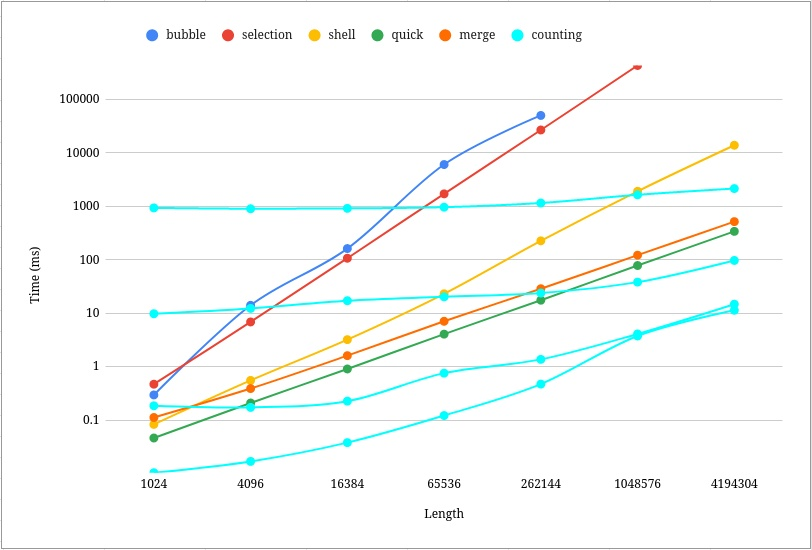
\includegraphics[scale=0.5]{1}	
			\caption{Графік (Час має логарифмічну шкалу)}
		\end{figure}
	
		\begin{figure}[H]
			\centering
			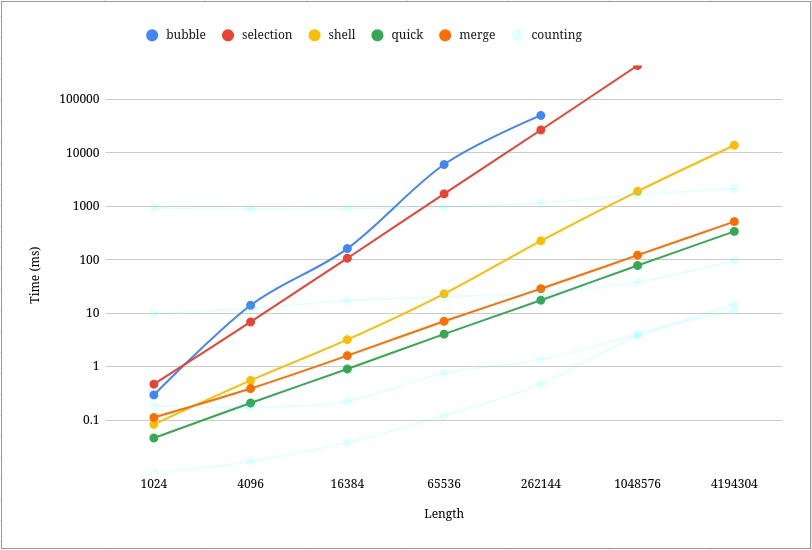
\includegraphics[scale=0.5]{2}	
			\caption{Графік (Час має логарифмічну шкалу)}
		\end{figure}
		
		\begin{figure}[H]
			\centering
			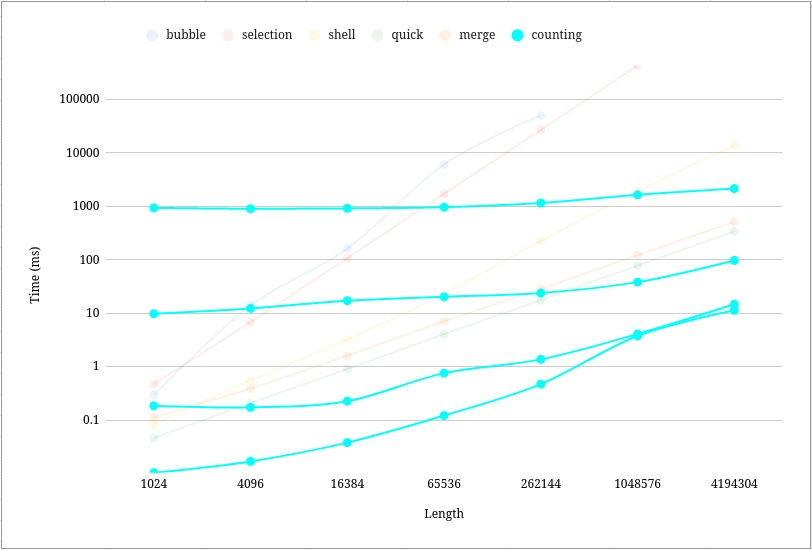
\includegraphics[scale=0.5]{3}	
			\caption{Графік (Час має логарифмічну шкалу)}
		\end{figure}
	
		\begin{figure}[H]
			\centering
			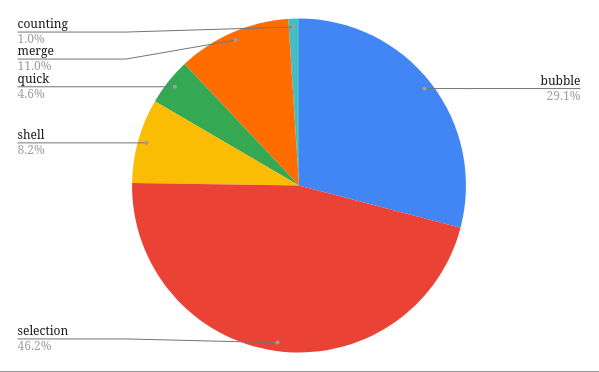
\includegraphics[scale=0.5]{4}	
			\caption{Секторна діаграма}
		\end{figure}
		
		\section*{Висновоки}
		Під час виконання лабораторної роботи я порівняв попередньо вивчені алгоритми сортування. Тестові дані складаються з масивів розміром 1024, 4096, 16384,  65536, 262144, 1048576, 4194304 цілочисельних елементів. В результаті аналізу я зробив наступні висновки:
		\begin{list}{•}{}
			\item \textbf{Алгоритм бульбашки} є найпростішим алгоритмом сортування, але водночас найповільнішим, оскільки складність алгоритму в усіх випадках складає $O(n^2)$. Порівняно з іншими алгоритмами бульбашка працює повільніше в сотні разів.
			
			\item \textbf{Алгоритм простої вибірки} також є досить неефективним алгоритмом сортування. Проте, даний алгоритм використовує набагато менше перестановок елементів, ніж бульбашка і складність змінюється від $O(n^2)$ до $O((n\cdot (n-1))/2)$. Отже, цей алгоритм працює дещо швидше за бульбашку, але все ще набагато повільніше ніж наступні алгоритми.
			
			\item \textbf{Алгоритм сортування Шелла}. Складність алгоритму в варіюється від $O(n^2)$ до $O(n\cdot\log\cdot n)$ залежно від розбиття на $gap$. В порівнянні з простими алгоритмами сортування, сортування Шелла працює достатньо швидко для масивів невеликого розміру, однак повільніше за наступні алгоритми для масивів більшого розміру.
			
			\item \textbf{Алгоритм швидкого сортування} має складність $O(n^2)$ однак на практиці наближається до $O(n\cdot \log n)$. Цей алгоритм показав найкращі результати для масиву в загальному випадку.
			
			\item \textbf{Алгоритм сортування злиттям} також є одним з найкращих алгоритмів, оскільки він працює за $O(n\cdot \log n)$  у всіх випадках. Проте він потребує виділення додаткової пам’яті, на практиці сортування злиттям показало результати дещо гірші за метод швидкого сортування.
			
			\item \textbf{Алгоритм сортування підрахунком} показав найкращий результат за умови, що вхідні дані є масивом цілих чисел з невеликим розмахом значень елементів. Даний алгоритм працює за лінійну складність $O(n+k)$.
		\end{list}

		Отже, в результаті аналізу я виявив, що алгоритм швидкого сортування є найкращим в загальному випадку, а алгоритм сортування підрахунком є найефективнішим для масивів з невеликим розмахом значень елементів і показує в сотні разів кращі результати для масивів великого розміру.
		
	\end{normalsize}
\end{document}
